\chapter{Introduction}
\label{sec:Introduction}


\section{Aim of \opal and History}
\opal is a tool for charged-particle optics in
accelerator structures and beam lines. 
Using the \mad language with extensions, \opal is derived from \madninep and is based 
on the
\htmladdnormallink{CLASSIC}{http://wwwslap.cern.ch/classic/} class library,
which was started in 1995 by an international collaboration.  IPPL (Independent Parallel Particle Layer) is
the framework which provides parallel particles and fields using data parallel ansatz. 
\opal is built from the ground up as a parallel application exemplifying the fact that HPC (High Performance Computing) 
is the third leg of science, complementing theory and the experiment. 
HPC is made possible now through the increasingly sophisticated mathematical models and evolving computer power available on the desktop
and in super computer centres. \opal runs on your laptop as well as on the largest HPC clusters available today. 

The \opal framework makes it easy to add new features in the form of new
\texttt{C++}~classes.

OPAL comes in the following flavours:
\begin{itemize}
\item \opalmap (not yet released in V1.0)
\item \opalcycl 
\item \opalt .
\end{itemize}

\opalmap tracks particles with 3D space charge using split operator techniques, and is a proper subset of \madninep. In the future 
a linear space charge mode will become available available
allowing the user to track moments of the distribution. 

\opalcycl tracks particles with 3D space charge including neighbouring turns in cyclotrons
with time as the independent variable. 

\opalt is a superset of IMPACT-T \cite{qiang2005} and can be used to model guns, injectors and complete XFEL's excluding the undulator.

It should be noted that not all features of \opal are available in all flavours.\\ The following icon \noopalt means that a feature is not yet 
available in \opalt. Similar icons are used for the other flavours. 

\section{Parallel Processing Capabilities}
\opal is built to harness the power of parallel processing for an improved quantitative understanding
of particle accelerators.
This goal can only be achieved with
detailed 3D modelling capabilities and a sufficient number of simulation particles to obtain meaningful statistics on various 
quantities of the particle ensemble such as emittance, slice emittance, halo extension etc. 

As a consequence the \opal architecture is based on data parallelism from the ground up while following the shared memory paradigm. 

\begin{table}[ht]
\caption{Parameters Parallel Performance Examples }
   \label{tab:drift}
\centering % used for centering table
\begin{tabular}{c c c c c c} % centered columns (4 columns)
\hline\hline %inserts double horizontal lines
Test & Particles  & Mesh & Greens Function & Time steps  \\ [0.75ex] % inserts table
%heading
\hline % inserts single horizontal line
PPE1 & $10^6$ & $128^3$ & Integrated  & 100 \\ [1ex] % inserting body of the table
\hline %inserts single line
\end{tabular}
\label{table:nonlin} % is used to refer this table in the text
\end{table}

In Figure \ref{fig:walldrift} the $W_{all}$ time as a function of used processors is shown for a test example. The simulation parameters for {\em PPE1 (Parallel Performance Example 1)}  are given in 
Table \ref{tab:drift}.
\begin{figure}[ht]
 \begin{center}
 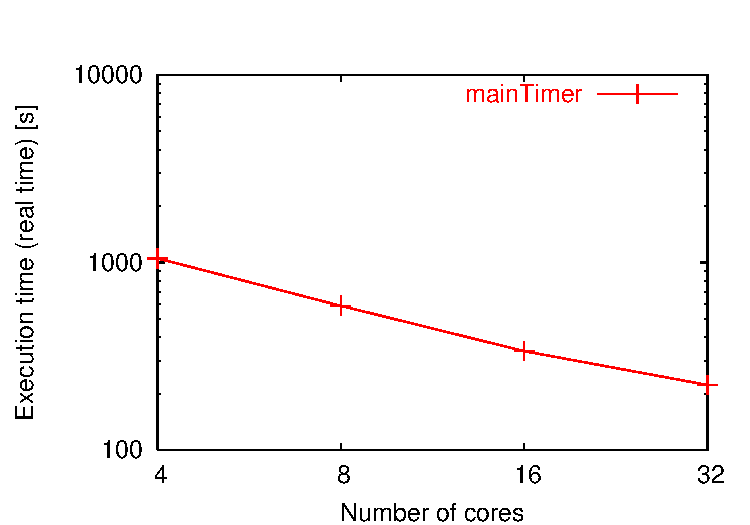
\includegraphics[width=0.5\linewidth,angle=0]{figures/speedup/Drift/mainTimer}
  \caption{$W_{all}$ time as a function of cores}
  \label{fig:walldrift}
 \end{center}
\end{figure}

In Figure \ref{fig:speedupdrift} speedup for PPE1 is shown. \latermore .

\begin{figure}[ht]
 \begin{center}
  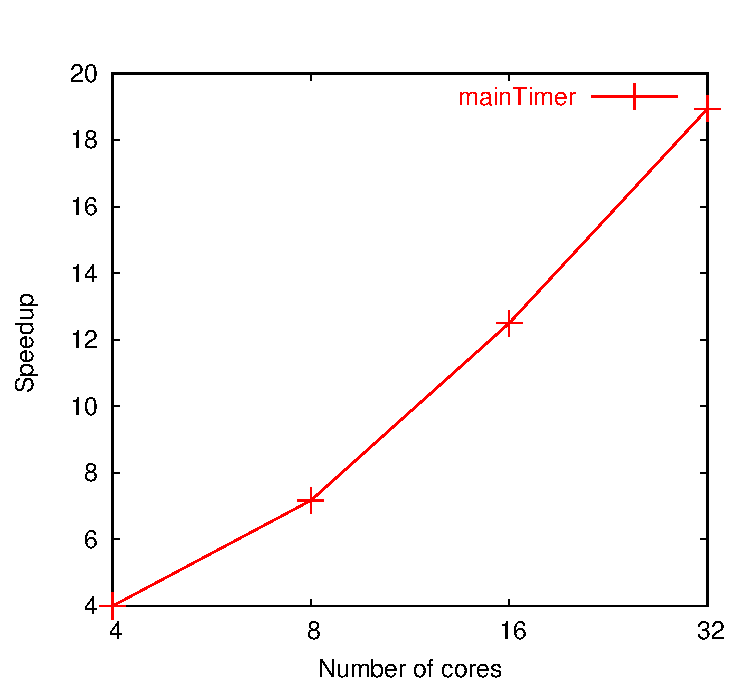
\includegraphics[width=0.6\linewidth,angle=0]{figures/speedup/Drift/mainTimer-speedup}
  \caption{Speedup as a function of used cores}
   \label{fig:speedupdrift}
 \end{center}
\end{figure}

\section{Quality Management}
Documentation and quality assurance are given our highest attention since we are convinced that adequate documentation 
is a key factor in the usefulness of a code like \opal to study present and future particle accelerators. 
 Using tools such as a source code version
control system (subversion), source code documentation (Doxygen, check out, for instance,  \url{http://amas.web.psi.ch/docs/opal/html/classParallelTTracker.html}) and the extensive user maunal
you are now enjoying, we are committed to providing users as well as co-developers with 
state-of-the-art documentation to \opal.

One example of an non trivial test-example is the PSI DC GUN. In Figure \ref{fig:guncomp1} the comparison between \impactt and \opalt is shown. This example is part of the regression test suite
that is run every night. The inputfile is found in Section \ref{sec:oblagun}.  
\begin{figure}[ht]
 \begin{center} 
   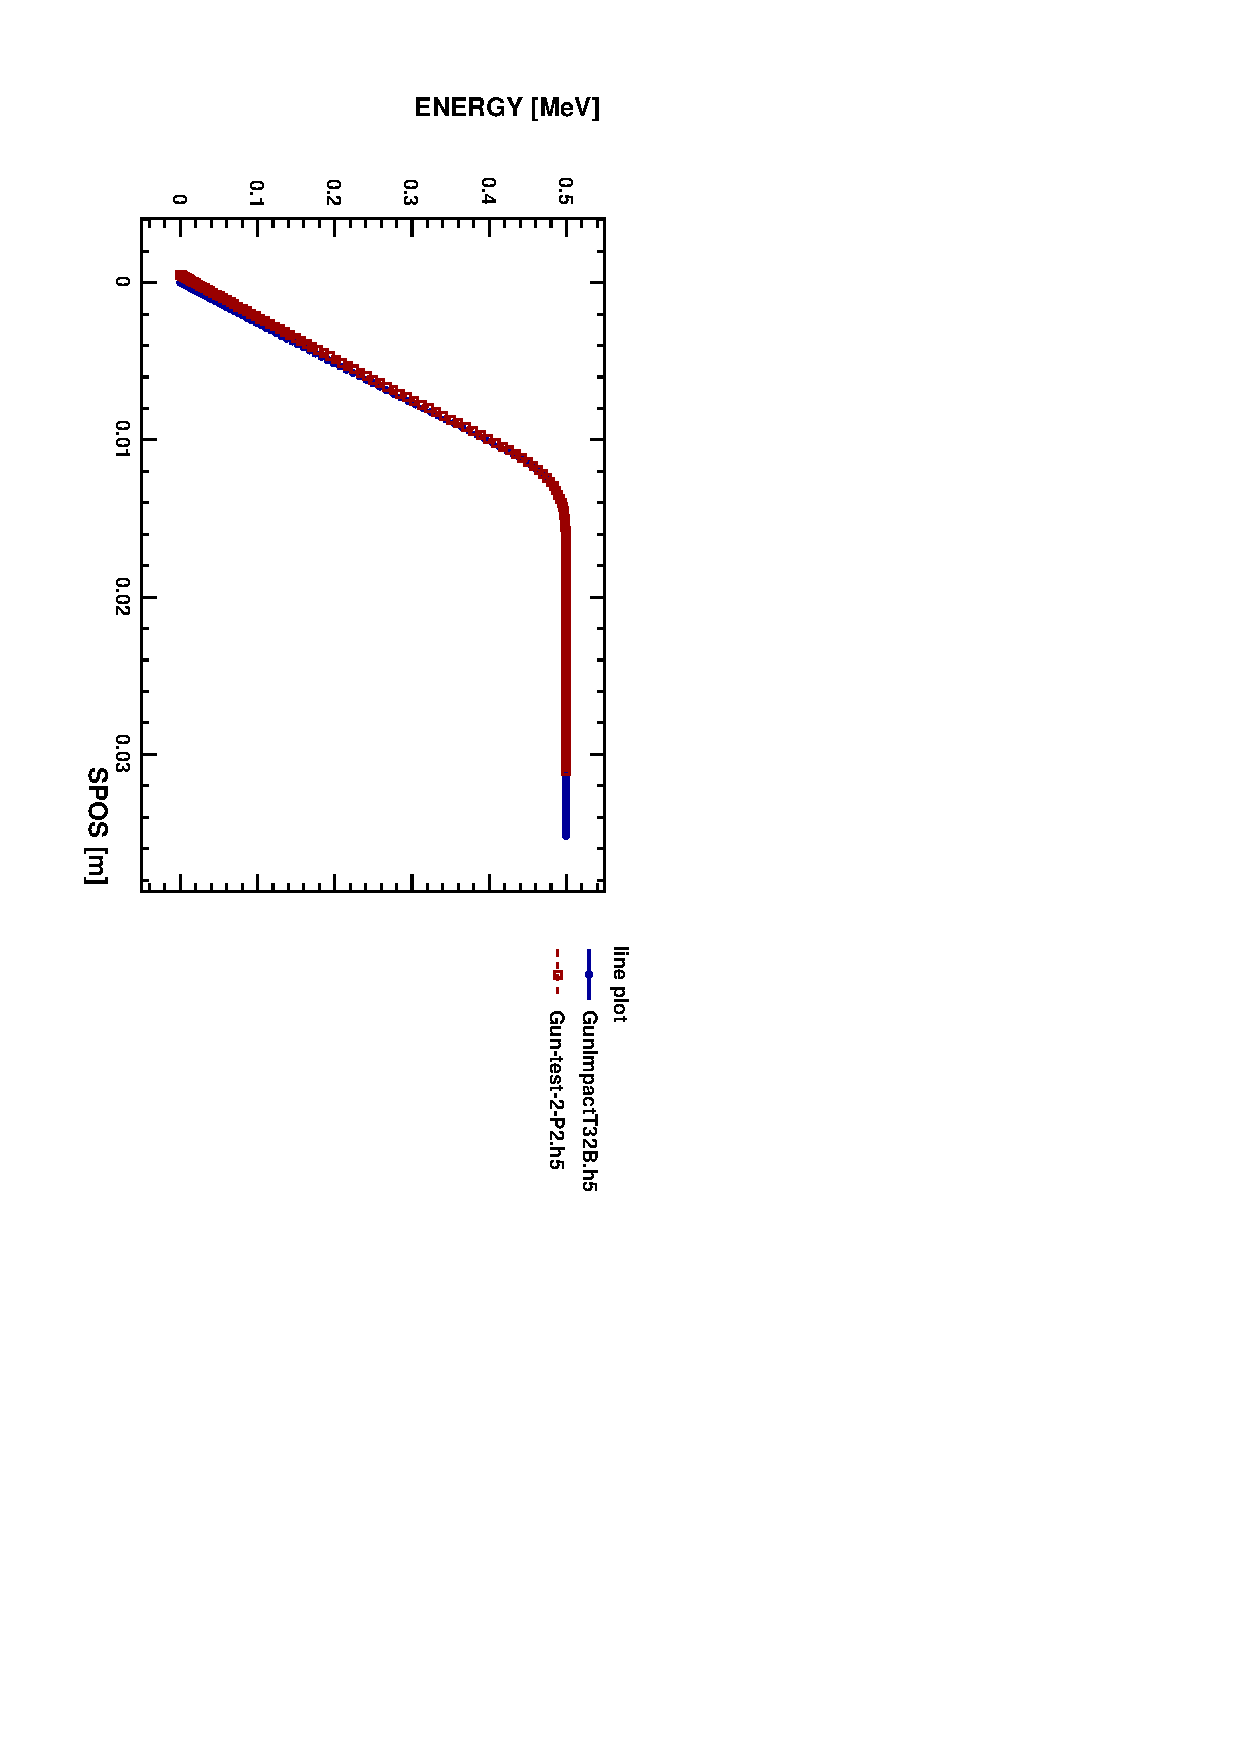
\includegraphics[width=0.60\linewidth,angle=90]{figures/Gun/GunCompEn}
   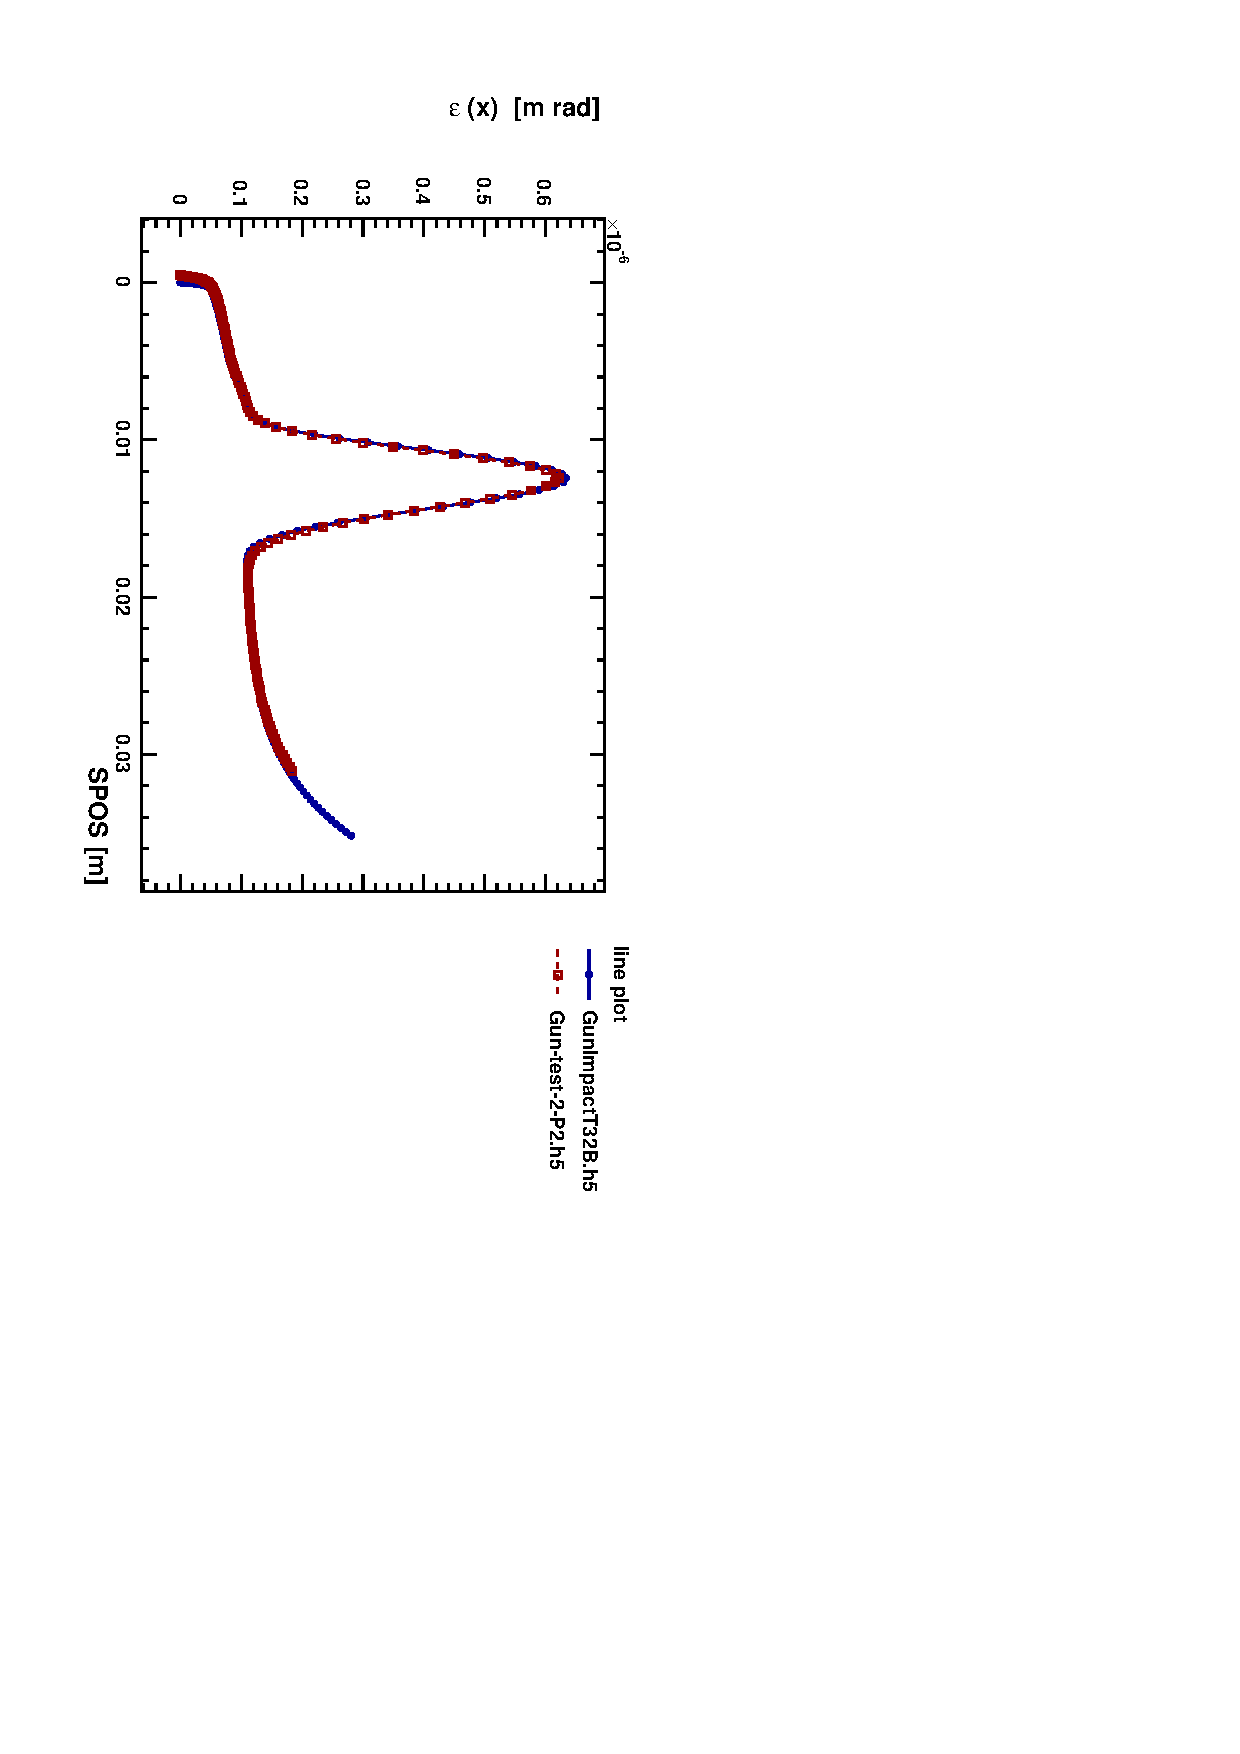
\includegraphics[width=0.60\linewidth,angle=90]{figures/Gun/GunCompEx}
   \caption{Comparison of energy and emittance in $x$ between \impactt and \opalt}   
   \label{fig:guncomp1}
 \end{center}
\end{figure}

\section{Revision 1.0 - Feature List}
\label{sec:featurelist}
In the current version of \opal many features have been implemented while others are still missing. 
Table~\ref{featurelist} lists the implemented features whereas Table~\ref{roadmap} outlines a rough road map to where we intend to bring \opal in the near and not so near future.
\begin{table}[ht] \footnotesize
\begin{center}
\begin{tabular}{p{5cm}cc}
\hline
{\bf Name} & {\bf implemented} & {\bf tested}\\
\hline
{\bf Algorithms} & & \\
ParallelTTracker & x & x \\
ParallelCyclotronTracker & x & x \\
FFT based space charge solver & x & x \\
integrated Greens function, FFT based space charge solver & x & x \\
\hline
{\bf Elements} & & \\
Cyclotron & x & x \\
RFCavity & x & x \\
Solenoid & x & x \\
Traveling Wave & x & x \\
Traveling Wave fast algorithm & x & x \\
RBend & x & \\
\hline
\end{tabular}
\caption{List of implemented and tested features in version 1.0 of \opal. For testing the output was compared to results of Impact-T.}
\label{featurelist}
\end{center}
\end{table}
\clearpage
\begin{table}[ht]\footnotesize
\begin{center}
\begin{tabular}{p{7cm}c}
\hline
{\bf Name} & {\bf Version (estimated)} \\
\hline
{\bf Algorithms} & \\
longitudinal and transverse wake fields& 1.1.x \\
ML based space charge solver & 1.1.x \\
1D csr wake fields & 1.1.x \\
2D FETD self-consistent solver & 1.2 \\
3D FETD self-consistent solver & 1.2 \\
\opalmap & 1.2 \\
\hline
{\bf Elements} &  \\
SBend & 1.1.x \\
Collimator & 1.1.x \\
\hline
\end{tabular}
\caption{List of features which will be implemented in versions to come (please note: the estimated version numbers are non-binding).}
\label{roadmap}
\end{center}
\end{table}
If there is any feature you are missing let us know. Alternatively you can check out the source code from our repository and implement it. In this case let us know and send a patch so that we can incorporate your work into \opal.
\clearpage
\section{Acknowledgements}
The contributions of various individuals and groups are acknowledged in the relevant chapters, however a few individuals have or had considerable influence on the 
development of \opal, namely Chris Iselin, John Jowett, Julian Cummings, Ji Qiang, Robert Ryne and Stefan Adam. For the \partroot visualisation tool credits go to Thomas Schietinger.
The effort to couple FEMAXX to \opal is led by Benedikt Oswald. 

Misprints and obscurity are almost inevitable in a document of this size.
Comments and {\em active contributions}  from readers are therefore most welcome.
They may be sent to \htmladdnormallink{\texttt{andreas.adelmann@psi.ch}}{mailto:andreas.adelmann@psi.ch}.


\subsection{Citation}
Please cite \opal in the following way:
\begin{small}
\begin{verbatim} 
@techreport{Opal-User-Guide,
title = "{The OPAL (Object Oriented Parallel Accelerator Library) 
              Framework }",
author = "A. Adelmann and Ch. Kraus and Y. Ineichen and  J. Yang",
institution = "Paul Scherrer Institut",
number = "PSI-PR-08-02",
year ={2008}
\end{verbatim}
\end{small}


%& OPAL \\
% & V 1.0


